\begin{abcliste}
\abc Each spectator is up for $\tau$; in that time the wave moves on by its width:
\begin{align}
 b &= \bwF = \v\times\tu = \bw \approx \result{\bwP{0}{2}}
\end{align}

\abc
\begin{align}
 t &= \tlF = \frac{\Cs}{\v} = \tl \approx \result{\tlP{0}{2}}
\end{align}

\abc The head rises once and comes down again within \tuO, and then stays at rest: a single bump, not a step and not a periodic motion.
\begin{center}
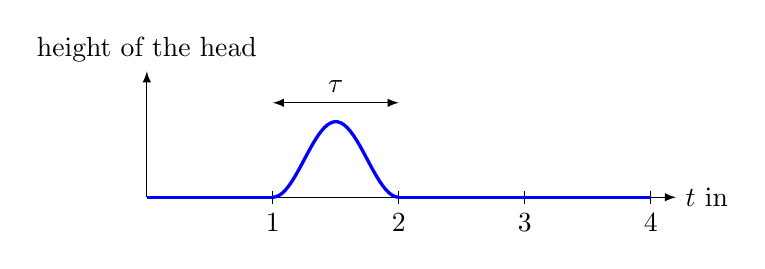
\begin{tikzpicture}[>=latex, x=1.6cm, y=1.6cm]
 \draw[->] (0,0) -- (4.2,0) node[right] {$t$ in \si{\s}};
 \draw[->] (0,0) -- (0,1) node[above] {height of the head};
 \foreach \t in {1,2,3,4} \draw (\t,0.05) -- (\t,-0.05) node[below] {\t};
 \draw[very thick, blue] (0,0) -- (1,0);
 \draw[very thick, blue, domain=1:2, samples=40] plot (\x, {0.6*sin(deg(pi*(\x-1)))^2});
 \draw[very thick, blue] (2,0) -- (4,0);
 \draw[<->] (1,0.75) -- node[above] {$\tau$} (2,0.75);
\end{tikzpicture}
\end{center}
Nobody runs round the stadium: each spectator only moves up and down, a moment after the neighbour. The wave is the pattern that moves.
\end{abcliste}
